% 第 6 章 Restriction Theorems (原书第 101-113 页)
\chapter{限制性定理}
\label{chap:6}

本章的目的是证明 Bochner--Riesz 算子 $T_\lambda$ 在最优范围 $\frac{2n}{n+1+2\lambda}\leq p\leq\frac{2n}{n-1-2\lambda}$ 内的 $L^p$ 有界性, 但仅当 $\lambda$ 相当大时如此. 问题在于控制振荡: 在一维情形, 我们曾把卷积核 $\frac{\sin 2\pi x}{x}$ 换成 $\frac{1}{x}$, 但在更高维数, 指数 $e^{i|x|}$ 无法简化. 我们将叙述 C.~Fefferman 与 E.~M.~Stein 的理论, 它分析的正是这类振荡核.

\section{限制}
\label{sec:6.1}
\index{限制性定理 (restriction theorem)|emph}

为了导出振荡效应的一个简单模型, 我们分析 $\mathbb{R}^{2}$ 中的一个简单的核:
\[
K(x)=\frac{e^{i|x|}}{|x|^{\frac{3}{2}+\lambda}}.
\]
设 $f$ 紧支集在 $D=\{y \mid |y|<1\}$ 中, 并设 $x$ 很大. 控制 $|x-y|$ 的几何如图~\ref{fig:4} 所示. 我们可以取 $|x-y|$ 近似等于 $|x|$ 减去 $y$ 在 $x$ 方向上的投影长度. 于是
\[
|x-y|\approx|x|-y\cdot\frac{x}{|x|},
\qquad
e^{i|x-y|}\approx e^{i|x|}\,e^{-iy\cdot\frac{x}{|x|}}.
\]
我们还可以估计
\[
|x-y|^{\frac{3}{2}+\lambda}\approx|x|^{\frac{3}{2}+\lambda}+\text{误差},
\]
于是
\begin{align*}
K\star f(x)=\int\frac{e^{i|x-y|}}{|x-y|^{\frac{3}{2}+\lambda}}\,f(y)\,dy
&\approx\frac{e^{i|x|}}{|x|^{\frac{3}{2}+\lambda}}\int e^{-iy\cdot\frac{x}{|x|}}\,f(y)\,dy \\
&=\frac{e^{i|x|}}{|x|^{\frac{3}{2}+\lambda}}\,\hat{f}\Bigl(\frac{x}{|x|}\Bigr).
\end{align*}
推论~\ref{cor:5.4} 的反例使我们预计 $T_{\lambda}f$ 会看起来像 $|x|^{-(\frac{3}{2}+\lambda)}$, 但这个新估计还要更好: 它把 $K$ 的作用分离成两个部分: 球面变量方向上的一个 Fourier 变换, 与无穷远处一个纯径向的衰减. 在极坐标下, 我们于是预计
\begin{align*}
\|K\star f\|_{p}^{p}&\geq\int_{2}^{\infty}\int_{0}^{2\pi}|K\star f(r,\theta)|^{p}\,d\theta\,r\,dr \\
&=\int_{2}^{\infty}r\,r^{-(\frac{3}{2}+\lambda)p}\,dr\cdot\int_{0}^{2\pi}\bigl|\hat{f}(1,\theta)\bigr|^{p}\,d\theta.
\end{align*}
由此可知, 除非 $p>\frac{4}{3+2\lambda}$, 否则 $K\star f$ 不属于 $L^p$; 若这一点满足, 则 $K$ 的 $L^p$ 有界性将蕴含
\[
\int_{0}^{2\pi}\bigl|\hat{f}(1,\theta)\bigr|^{p}\,d\theta\leq C\|f\|_{p}^{p}.
\]
这种类型的不等式称为\emph{限制性定理} (restriction theorem), 因为它支配着 $f$ 的 Fourier 变换在集合 $\{\xi \mid |\xi|=1\}$ 上的限制, 而这毕竟是一个零测集. 这是了不起的, 因为任意的可测函数是无法限制到零测集上而不出现无穷的. 另一方面, 若 $f\in L^p$, $1<p\leq 2$, 则 $\hat{f}$ 是由 $L^{p'}$ 范数中的极限过程计算的: 若 $f_n\in\mathcal{S}$ 且 $f_n\to f$, 则 Hausdorff--Young 不等式
\[
\|\hat{f}\|_{p'}\leq\|f\|_{p}
\]
保证诸 $\hat{f}_n$ 按 $L^{p'}$ 范数收敛到某个函数 $\hat{f}$. 一个子列几乎处处收敛, 于是 $\hat{f}$ 几乎处处有定义. 但在一个零测集上定义 $\hat{f}$ 看起来是荒谬的.

\begin{figure}[htbp]
\centering
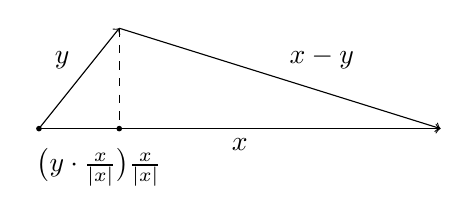
\begin{tikzpicture}[scale=0.85]
  % 小球 D 与向量 y
  \fill (0,0) circle (1.2pt);
  \draw[->] (0,0) -- (1.2,1.5) node[midway, above left] {$y$};
  \draw[->] (0,0) -- (6,0) node[midway, below] {$x$};
  \draw[->] (1.2,1.5) -- (6,0) node[midway, above right] {$x-y$};
  % 投影虚线
  \draw[dashed] (1.2,1.5) -- (1.2,0);
  \fill (1.2,0) circle (1.2pt);
  \node[below] at (0.9,-0.15) {$\bigl(y\cdot\frac{x}{|x|}\bigr)\frac{x}{|x|}$};
\end{tikzpicture}
\caption{球面上两点间距离与法向几何}
\label{fig:4}
\end{figure}

由于限制性定理令人惊讶到使人怀疑其正确性, 并让人对 $T_{\lambda}$ 的有界性起疑, 我们就从限制性定理讲起.

\begin{proposition}\label{prop:6.1}
设 $f$ 是 $\mathbb{R}^n$ 上的径向函数. 则
\[
\bigl|\hat{f}(1,\theta)\bigr|\leq C\|f\|_{p}
\]
对 $L^p$ 中所有的径向 $f$ 成立, 当且仅当 $1\leq p<\frac{2n}{n+1}$.
\end{proposition}

\begin{proof}
由于 $f$ 径向, $\hat{f}$ 也径向, 于是 $\hat{f}(1,\theta)$ 与 $\theta$ 无关. 那么线性泛函 $f\mapsto\hat{f}(1,\theta)$ 在 $L^p$ 上有界当且仅当它由对一个 $L^{p'}$ 函数的积分给出. 我们把 $\hat{f}(1,\theta)$ 缩写为 $\hat{f}(1)$; 则
\begin{align*}
\hat{f}(1)&=\int_{0}^{\infty}f(r)\int_{S^{n-1}}e^{2\pi i\sigma r\xi}\,d\sigma\,r^{n-1}\,dr \\
&=\int_{0}^{\infty}f(r)\,\frac{J_{\frac{n-2}{2}}(2\pi r|\xi|)}{(r|\xi|)^{\frac{n-2}{2}}}\,r^{n-1}\,dr.
\end{align*}
但
\[
\frac{J_{\frac{n-2}{2}}(2\pi r)}{r^{\frac{n-2}{2}}}
\]
属于 $L^{p'}$ 当且仅当 $p'>\frac{2n}{n-1}$. 结论得证.
\end{proof}

这只是通往定理的一个初步近似, 因为它只处理径向函数. 尽管如此, 它表明即便是这些函数的 Fourier 变换也具有令人惊讶的光滑性 (在一定程度上). 下一个结果试图对限制中出现的临界指标 $\frac{2n}{n+1}$ 给出一个几何层面的理解; 我们想限制从 $L^p$ 到 $L^q$ 的限制性可能成立的 $(p,q)$ 的范围. 我们关于 Fourier 变换最初得到的估计是在 Hausdorff--Young 定理中; 我们利用 Fourier 变换的伸缩结构证明了这些估计是最优的: $f(\delta x)$ 被变换为 $\delta^{-n}\hat{f}(\delta^{-1}\xi)$. 但圆对伸缩并不是不变的, 我们必须更狡猾一些.

直观上, 我们想让 $\hat{f}|_{S^1}$ 尽可能大. 利用伸缩, 我们设想 $\hat{f}$ 支在一个小矩形上, 并把它定向为与 $S^1$ 相交尽可能多. 见图~\ref{fig:5}. 支集 $\hat{f}$ 的什么样的尺寸能在最小化 $\|f\|_p$ 的同时最大化 $\hat{f}|_{S^1}$? 取矩形的大小为 $\delta\times\delta^{\alpha}$, 其中 $\alpha<1$, 从而这是长边. 我们选取 $\alpha$ 使得矩形的角恰好与圆相交; 这使与圆的相交达到最大. 由于 $x=\sqrt{1-y^2}=\sqrt{1-(1-\delta)^2}\approx\sqrt{\delta}$, 我们取 $\alpha=\frac{1}{2}$.

\begin{figure}[htbp]
\centering
\begin{tikzpicture}[scale=0.85]
  % 圆弧 (大半径圆的一段)
  \draw (-3.4,-1.2) arc (250:290:9);
  % 矩形
  \draw (0,0) rectangle (4.5,-1.2);
  \node[above] at (2.25,0.05) {$\delta^{\alpha}$};
  \node[right] at (4.55,-0.6) {$\delta$};
\end{tikzpicture}
\caption{Knapp 反例函数的支撑集几何}
\label{fig:5}
\end{figure}

% 原书编号由 6.1 直接跳至 6.3, 此处跳过 6.2 以与原书一致.
\addtocounter{mtthm}{1}

\begin{proposition}\label{prop:6.3}
不等式
\[
\|\hat{f}|_{S^{n-1}}\|_{q}\leq C\|f\|_{p}
\]
在 $q>\frac{n-1}{n+1}p'$ 时不成立.
\end{proposition}

\begin{proof}
设 $\psi$ 是光滑的紧支集函数, 满足当 $|\xi|<\sqrt{n}$ 时 $\psi(\xi)=1$. 定义
\[
\hat{f}_{\delta}(\xi_{1},\ldots,\xi_{n})=\psi\bigl(\delta^{-2}(\xi_{1}-1),\,\delta^{-1}\xi_{2},\,\ldots,\,\delta^{-1}\xi_{n}\bigr).
\]
若 $\delta<1$, $\xi\in S^{n-1}$, $|\xi_j|\leq\frac{\delta}{\sqrt{n}}$, 我们断言 $\hat{f}_\delta=1$. 只需证 $\delta^{-2}|\xi_1-1|<1$, 即 $1-\xi_1<\delta^2$. 但
\begin{align*}
1-\xi_{1}&=1-\sqrt{1-(\xi_{2}^{2}+\cdots+\xi_{n}^{2})}
\leq 1-\bigl(1-(\xi_{2}^{2}+\cdots+\xi_{n}^{2})\bigr) \\
&=\xi_{2}^{2}+\cdots+\xi_{n}^{2}\leq(n-1)\left(\frac{\delta}{\sqrt{n}}\right)^{2}\leq\delta^{2}.
\end{align*}
因此,
\begin{align*}
\|\hat{f}|_{S^{n-1}}\|_{q}
&\geq\left|\{(\xi_{1},\ldots,\xi_{n}) \mid |\xi_{j}|\leq\frac{\delta}{\sqrt{n}}\}\right|^{\frac{1}{q}}
\geq C\left(\frac{\delta}{\sqrt{n}}\right)^{\frac{n-1}{q}}
=C\delta^{\frac{n-1}{q}}.
\end{align*}
另一方面,
\[
f_{\delta}(x_{1},\ldots,x_{n})=\delta^{n+1}e^{2\pi ix_{1}}\,\check{\psi}(\delta^{2}x_{1},\,\delta x_{2},\,\ldots,\,\delta x_{n}),
\]
于是
\[
\|f_{\delta}\|_{p}=\delta^{\frac{n+1}{p'}}\|\check{\psi}\|_{p}=C\delta^{\frac{n+1}{p'}}.
\]
这样, 对所有小的 $\delta$, 有 $\delta^{\frac{n+1}{p'}}\geq C\delta^{\frac{n-1}{q}}$, 定理随之得证.
\end{proof}

\begin{remark}\label{rem:6.4}
在图~\ref{fig:6} 中, 我们画出了已知限制性失效的区域. 虚线表示上述结果中区域的边界; 竖直线来自要求 $1\leq p<\frac{2n}{n+1}$, 即便对径向函数这也是必要的. 两条线相交于 $p=q=\frac{2n}{n+1}$.
\end{remark}

\begin{figure}[htbp]
\centering
\begin{minipage}[b]{0.45\textwidth}
\centering
\begin{tikzpicture}[scale=0.75]
  % 图 6: 失效区域 (斜线阴影在虚线上方/左侧)
  \fill[pattern=north west lines, pattern color=black!70]
    (0,0) -- (0,4.2) -- (3.1,4.2) -- (3.1,3.1) -- (4.2,0) -- cycle;
  \draw (0,0) rectangle (4.2,4.2);
  \draw[dashed] (3.1,3.1) -- (4.2,0);
  \draw (3.1,0) -- (3.1,4.2);
  \fill (3.1,3.1) circle (2.2pt);
  \fill (4.2,0) circle (2.2pt);
  \node[right] at (4.3,3.1) {$\frac{n+1}{2n}$};
  \node[below] at (3.1,-0.2) {$\frac{n+1}{2n}$};
  \node[below=0.5cm] at (2.1,-0.3) {};
\end{tikzpicture}
\caption{限制性估计失效的指标区域}
\label{fig:6}
\end{minipage}\hfill
\begin{minipage}[b]{0.45\textwidth}
\centering
\begin{tikzpicture}[scale=0.75]
  % 图 7: 有界区域 (斜线阴影在右上方窄条)
  \fill[pattern=north west lines, pattern color=black!70]
    (3.1,4.2) -- (3.1,2.3) -- (4.2,0) -- (4.2,4.2) -- cycle;
  \draw (0,0) rectangle (4.2,4.2);
  \draw[dashed] (3.1,4.2) -- (3.1,2.3);
  \draw (3.1,2.3) -- (4.2,0);
  \draw (3.1,2.3) circle (2.2pt);
  \fill (3.5,1.15) circle (2.2pt);
\end{tikzpicture}
\caption{Tomas--Stein 限制性有界区域}
\label{fig:7}
\end{minipage}
\end{figure}

\begin{proposition}\label{prop:6.5}
\index{球面测度 (surface measure $d\sigma$)}
若 $1\leq p\leq\frac{2(n+1)}{n+3}$, 则
\[
\|\hat{f}|_{S^{n-1}}\|_{2}\leq C\|f\|_{p}.
\]
\end{proposition}

\begin{proof}
我们可以假设 $f\in\mathcal{S}$, 这为下面的形式运算提供了依据. 则
\begin{align*}
\|\hat{f}|_{S^{n-1}}\|_{2}^{2}
&=\int\hat{f}(\sigma)\,\overline{\hat{f}(\sigma)}\,d\sigma
=\int(f\star\tilde{f})\,\widehat{d\sigma}
=\int f\star\tilde{f}(x)\,\widehat{d\sigma}(x)\,dx \\
&=\int\check{d\sigma}\star f(x)\,f(x)\,dx
\leq\|f\|_{p}\,\|\check{d\sigma}\star f\|_{p'}.
\end{align*}
只需证明 $Rf=\check{d\sigma}\star f$ 是从 $L^p$ 到 $L^{p'}$ 的有界映射. 我们有两种技术: 一是把 $\check{d\sigma}(x)$ 切成碎块; 二是使用复内插. 这里我们做内插; 在定理之后的讨论中, 我们会看到标准模型能告诉我们什么.

我们需要把算子 $R$ 嵌入一个解析的算子族; 令 $R_{z}f=K_{z}\star f$; 照例, 我们只能控制在 $p=1$ 与 $p=2$ 处发生的事情. 于是在 $p'=\infty$ 与 $p'=2$ 处, 我们用
\begin{align*}
\|K_{z}\star f\|_{\infty}&\leq\|K_{z}\|_{\infty}\,\|f\|_{1}, \\
\|K_{z}\star f\|_{2}&\leq\|\hat{K}_{z}\|_{\infty}\,\|f\|_{2}.
\end{align*}
啊, 又是我们的老对手——对 $K$ 与 $\hat{K}$ 的同时控制! 现在,
\[
K_{0}=\widehat{d\sigma}(x)=\frac{J_{\frac{n-2}{2}}(2\pi|x|)}{|x|^{\frac{n-2}{2}}},
\]
它不仅属于 $L^\infty$, 而且 $|x|^{\frac{n-1}{2}}K_0\in L^\infty$. 所以, 我们可以容许把 $K_0$ 弄得更糟一些而仍保持第一个不等式. 另一方面, $\hat{K}_0=d\sigma$, 它根本不是一个 $L^\infty$ 函数, 所以必须对它作相当大的改进. 在改进与变糟之间将落下 $K_z$, 而我们将得到一个使 $K_0$ 给出有界算子的 $p$ 的范围. 令
\[
K_{z}(x)=c_{z}\frac{J_{\frac{n-2}{2}+z}\bigl(2\pi|x|\bigr)}{|x|^{\frac{n-2}{2}+z}}.
\]
若 $z=-\frac{n-1}{2}$, 则 $\frac{n-2}{2}+z=-\frac{1}{2}$, 并且由 Watson 的公式 3.4(6) 我们注意到
\[
J_{-\frac{1}{2}}(2\pi|x|)=\frac{\cos 2\pi|x|}{(\pi|x|)^{\frac{1}{2}}}.
\]
于是, 在 $z=-\frac{n-1}{2}$ 处, $K_z\in L^\infty$ (事实上, 这正是我们从 Bessel 函数的渐近性所预期的).

另一方面, 若 $z>0$, 则 $\hat{K}_z(\xi)=(1-|\xi|^2)_+^{z-1}$, 它首次属于 $L^\infty$ 是在 $z-1=0$ 时. 复内插给出 $z=\frac{n+3}{2}-\frac{n+1}{p}$. 在 $z=0$ 处, 这就给出定理.
\end{proof}

\begin{remark}\label{rem:6.6}
\begin{enumerate}[label=\alph*)]
\item 在图~\ref{fig:7} 中, 我们画出了限制性已知有界的区域. 空心圆与虚线表示已知无界的区域.
\item 若把 $f$ 换成 $\delta^{-n}f(\delta^{-1}x)$, 则 $\hat{f}$ 被换成 $\hat{f}(\delta\xi)$, 而 $\hat{f}_\delta|_{S^{n-1}}$ 与限制在半径为 $\delta^{-1}$ 的球面上的 $\hat{f}$ 相同. 把变量替换进行到底, 得到
\[
\left(\int_{S^{n-1}}\bigl|\hat{f}(R,\sigma)\bigr|^{2}\,d\sigma\right)^{\frac{1}{2}}
\leq C_{p}\,R^{-\frac{n}{p'}}\|f\|_{p}. \qedhere
\]
\end{enumerate}
\end{remark}

\essayhead{ess:6.7}{限制性再论}

利用标准模型可以证明一个较弱版本的限制性定理; 如同定理~\ref{thm:5.6} 的证明, 我们写 $\widehat{d\sigma}=\sum K_j$. 由于
\[
|\widehat{d\sigma}(x)|\leq C|x|^{-\frac{n-1}{2}},
\]
故
\[
\|K_{j}\|_{\infty}\leq C2^{-j\frac{n-1}{2}}.
\]
为估计 $\|\hat{K}_j\|_\infty$, 我们依靠~\ref*{prop:5.2} 中的想法: $\hat{K}_j=\psi_\delta\star d\sigma$, 其中 $\delta=2^{-j}$. 直观上, $\psi_\delta$ 紧支集在半径为 $\delta$ 的球中, 于是 $\psi_\delta\star d\sigma$ 在环形区域 $1-\delta<|\xi|<1+\delta$ 之外为零. 为使 $\psi_\delta\star d\sigma$ 达到最大, 我们看 $|\xi|=1$; 此时 $\psi_\delta\star d\sigma$ 应当被看作 $\psi_\delta$ 对 $d\sigma$ 的平均. 也就是说, 它是半径为 $\delta$ 的球在球面上的平均. 该球与球面相交处的曲面测度为 $\delta^{n-1}$; 而球本身的测度为 $\delta^n$, 于是这个平均是 $\delta^{-1}=2^j$. 因此我们预计:
\[
\|K_{j}\|_{\infty}\leq C2^{-j\frac{n-1}{2}},
\qquad
\|\hat{K}_{j}\|_{\infty}\leq C2^{j}.
\]
于是, 与 $K_j$ 作卷积的算子的范数是 $2^{\epsilon j}$, 其中
$\epsilon=2\bigl(1-\frac{1}{p}\bigr)-\frac{n-1}{2}\Bigl(1-2\bigl(1-\frac{1}{p}\bigr)\Bigr)$.
当 $p<2\frac{n+1}{n+3}$ 时它是负的.

用我们的标准模型解释限制性, 仍然没有告诉我们这一切究竟意味着什么. 我们将编织一个相当复杂的论证, 以展示使限制性得以成立的一些想法. 尽管如此, 时至今日仍无人能给出一个几何判别法, 来判定哪些零测集具有限制性而哪些没有, 所以我们很难说已经理解了限制性.

我们将首先考察曲率的影响. 若限制性对某条曲线 $S\subset\mathbb{R}^2$ 成立, 而 $S$ 包含一段线段, 则通过平移、旋转、伸缩与截断, 我们可以假设 $S=[0,1]\times\{0\}$. 现在令 $f(x_1,x_2)=g(x_1)h(x_2)$, 并注意 $\hat{f}(\xi_1,\xi_2)|_S=\hat{g}(\xi_1)|_I\,\hat{h}(0)$; 于是若取固定的 $g\in\mathcal{S}$ 使 $\hat{g}|_I=1$, 则限制性不等式将蕴含 $|\hat{h}(0)|\leq C\|h\|_{p}$. 于是映射 $h\mapsto\hat{h}(0)$ 是 $L^p$ 上的有界线性泛函, 这蕴含 $e^{2\pi i0x}\in L^{p'}$. 这只有在 $p=1$ 时才成立. 寓意是: 对任何包含一片超平面的曲面, 限制性都不可能成立.

我们的第二个观察把 $S$ 上的限制性与支在 $S$ 上的测度的 Fourier 变换联系起来. 设 $S$ 是光滑紧曲面, $d\sigma$ 为曲面测度; 我们断言: 不等式 $\|\hat{f}|_{S}\|_{q}\leq C\|f\|_{p}$ 对某个 $p>1$ 成立, 当且仅当 $\widehat{d\sigma}\in L^{p_0}$ 对某个 $p_0<\infty$ 成立.

先设限制性成立. 定义 $R:L^p(\mathbb{R}^n)\to L^q(S)$ 为 $Rf=\hat{f}|_S$. 则伴随算子 $R^{\star}:L^{q'}(S)\to L^{p'}(\mathbb{R}^n)$ 也有界, 并且我们很快可以算出
\begin{align*}
\int\bigl(R^{\star}g\bigr)(x)\,f(x)\,dx
&=\int g(\sigma)\,Rf(\sigma)\,d\sigma
=\int g(\sigma)\,\hat{f}(\sigma)\,d\sigma
=\int\widehat{g\,d\sigma}(x)\,f(x)\,dx.
\end{align*}
于是 $R^{\star}g=\widehat{g\,d\sigma}$; 这必须在分布的意义下理解, 而且就我们的目的而言, 不妨设 $g\in C^\infty(S)$. 取 $g\equiv 1$,
\[
\|\widehat{d\sigma}\|_{p'}\leq C|S|^{\frac{1}{q'}}.
\]
若 $p>1$, 则 $p'<\infty$.

反之, 设 $\widehat{d\sigma}\in L^{p_0}$ 对某个 $p_0<\infty$ 成立. 则
\[
\int|\hat{f}|^{2}\,d\sigma=\int f\star\widehat{f\,d\sigma}
\leq\|\widehat{d\sigma}\|_{p_{0}}\|f\star f\|_{p_{0}'}
\leq C\|f\|_{p}^{2};
\]
这里我们用了 Young 卷积不等式
\[
\|h\star g\|_{r}\leq\|h\|_{p}\,\|g\|_{q},
\qquad
1+\frac{1}{r}=\frac{1}{p}+\frac{1}{q}.
\]
由于 $r=p_{0}'$, $p=q$, 故 $p=\frac{2p_{0}}{2p_{0}-1}>1$.

既然 $d\sigma$ 的 Fourier 变换的 $L^p$ 行为刻画了 $S$ 的可限制性, 对限制性的几何理解就必须从``$S$ 的曲率如何影响 $\widehat{d\sigma}$ 的大小''开始. 正确的结果是: 若 $S$ 的曲率在 $S$ 的任何一点处都不无穷阶消失, 则 $\widehat{d\sigma}\in L^{p_0}$. 与其在这里试图证明它, 不如看看标准模型如何处理直线与圆的差别. 设 $\phi$ 是光滑函数, 当 $|x|<1$ 时 $\phi(x)=1$, 当 $|x|>2$ 时 $\phi(x)=0$. 则当 $\delta\to 0$ 时, $\delta^{-1}\phi(\delta^{-1}x_2)\phi(x_1)$ 按分布收敛到支在 $[-1,1]\times\{0\}$ 上的测度. 其 Fourier 变换的行为如同
\[
\hat{\phi}(\xi_{1})\,\check{\phi}(\delta\xi_{2})\to\hat{\phi}(\xi_{1})\check{\phi}(0)=\check{\phi}(\xi_{1}).
\]
由于在 $\xi_{2}$ 方向上完全没有衰减, 它不属于任何 $p<\infty$ 的 $L^{p}$.

那么单位圆有何不同? 我们有
\[
\lim_{\delta\to0}\delta^{-1}\psi\bigl(\delta^{-1}(|\xi|-1)\bigr),
\]
而且有估计
\[
\bigl|\bigl[\psi\bigl(\delta^{-1}(|\xi|-1)\bigr)\bigr]\check{}\,(x)\bigr|\leq C\delta\,|x|^{-\frac{n-1}{2}}\,\check{\psi}(\delta|x|).
\]
于是我们预计在极限中
\[
\bigl|\widehat{d\sigma}(x)\bigr|\leq C|x|^{-\frac{n-1}{2}},
\]
而这确实成立. 我们所缺乏的, 是对 $\check{\psi}$ 的估计的几何理解. 命题~\ref{prop:5.2} 中的计算始于 Bessel 函数的渐近性, 而当我们利用球面对称计算 $\widehat{d\sigma}$ 时, Bessel 函数又出现了. 这类公式唯一的问题在于它们平均得太多; 我们想要局部化. 我们从对 $\mathbb{R}^2$ 中一个环形区域的 Fourier 变换的几何理解开始.

\essayhead{ess:6.8}{重访``凸起''}
\index{曲率 (curvature)}

我们的问题在于: Fourier 变换非常适合把 $\mathbb{R}^2$ 看作一维空间的乘积; 计算矩形的变换很容易, 球则难一些. 因此, 若把一个环形区域分解成矩形, 计算会容易得多. 我们用单位分解把它分解成环状片段 $R_j$, 每个的大小为 $\sqrt{\delta}\times\delta$; 这给出 $\frac{2\pi}{\sqrt{\delta}}$ 块. 若 $v_j$ 表示顶点在 $R_j$ 中心的单位向量, 则 $v_j=(\cos\theta_j,\sin\theta_j)$, 其中 $\theta_j\approx j\sqrt{\delta}$. 我们可以把这些矩形视为以原点为中心的矩形 $R_j^0$ 的平移:
\[
\chi_{R_{j}}(\xi)=\chi_{R_{j}^{0}}(\xi-v_{j});
\qquad
\check{\chi}_{R_{j}}(x)=e^{2\pi iv_{j}x}\,\check{\chi}_{R_{j}^{0}}(x).
\]
为理解 $\check{\chi}_{R_{j}^{0}}(x)$, 我们把积分
\[
\int_{R_{j}^{0}}e^{2\pi ix\xi}\,d\xi
\]
看作让某些波对矩形作平均的过程. 在二维, 这些是沿方向 $\frac{x}{|x|}$ 传播、频率为 $|x|$ 的平面波. 哪些方向与哪些频率对 $\chi_{R_j^0}$ 的 Fourier 变换有贡献?

若方向平行于 $v_j$, 即 $x=v_j|x|$, 则波对一个厚度为 $\delta$ 的区间作平均, 于是使这种平均非零的适当频率是 $|x|=\delta^{-1}$. 此时平均给出矩形的大小, 即 $\delta^{\frac{3}{2}}$, 因而这个频率与方向贡献 $e^{2\pi ixv_j}\delta^{\frac{3}{2}}$. 但 $x=v_j|x|$, $|x|=\delta^{-1}$, 于是我们得到大小为
\[
\frac{e^{2\pi i|x|}}{|x|^{\frac{3}{2}}}
\]
的贡献.

那么还有哪些方向有贡献? 在 $\pi$ 方向, 我们得到与 $0$ 方向同样大小的贡献, 但相位不同, 于是求和给出一个余弦. 在垂直于 $v_j$ 的方向, 进来的波``看到''的厚度是 $\sqrt{\delta}$, 于是它挑选频率 $|x|=\delta^{-\frac{1}{2}}$, 其中 $x=|x|w_j$, $v_j\cdot w_j=0$. 这样的波对 Fourier 变换的贡献是 $\delta^{\frac{3}{2}}=|x|^{-\frac{3}{2}}$. 由于这小得多, 我们采取这样的直观: 凡是不平行于 $v_{j}$ 的方向都可以忽略, 尽管这当然是非常简化的. 总而言之,
\[
\check{\chi}_{R_{j}}(x)=\frac{e^{2\pi i|x|}}{|x|^{\frac{3}{2}}}.
\]
现在为计算 $\psi_\delta$, 我们需要把来自诸 $R_j$ 的贡献加起来. 它们会在 $x$ 一侧相互作用, 我们需要控制这一点. 直观上, 我们把 $R_j^0$ 想成在 $v_j$ 与 $w_j$ 方向上的矩形, 于是其 Fourier 变换又是一个矩形 $S_j$, 在 $w_j$ 方向上大小为 $\delta^{-\frac{1}{2}}$, 在 $v_j$ 方向上大小为 $\delta^{-1}$. 我们断言这些矩形本质上互不重叠. 诸 $S_j$ 与原点的距离为 $|x|=\delta^{-1}$, 而相邻矩形之间的夹角为 $C\delta^{\frac{1}{2}}$. 于是, 中心之间的距离为
\[
\delta^{-1}\,\delta^{\frac{1}{2}}=\delta^{-\frac{1}{2}}
\]
(在 $w_j$ 方向). 这样 $S_j$ 与 $S_{j+1}$ 本质上不相交, 而且随着 $j$ 的变动, 整个环形区域被诸 $S_j$ 覆盖. 我们得出结论:
\[
\check{\psi}_{\delta}(x)=\frac{\cos 2\pi|x|}{|x|^{\frac{3}{2}}},
\qquad |x|\approx\delta^{-1}.
\]
把诸 $\psi_{2^{-j}}$ 加起来便得到 $\chi_{D}$, 或者取极限便得到 $\check{d\sigma}$.

\section{Bochner--Riesz 平均}
\label{sec:6.2}

\begin{theorem}\label{thm:6.9}
若 $\lambda>\frac{n-1}{2(n+1)}$, 则对最优范围
\[
\frac{2n}{n+1+2\lambda}<p<\frac{2n}{n-1-2\lambda},
\]
$T_\lambda$ 在 $L^p(\mathbb{R}^n)$ 上有界.
\end{theorem}

\begin{proof}
我们像之前那样分解 $K_{\lambda}=\sum K_j$, 但不做内插, 而是采用这样的哲学: $\hat{K}_j=\psi_\delta\star\mu_\lambda$ 的行为如同集中在厚度为 $\delta$ 的环形区域上. 于是~\ref*{rem:6.6}b) 控制了到这类环形区域上的限制:
\begin{align*}
\|K_{j}\star f\|_{2}^{2}&=\|\hat{K}_{j}\hat{f}\|_{2}^{2}
=\int_{1-\delta<|\xi|<1+\delta}|\mu_{\lambda}(\xi)|^{2}\,\bigl|\hat{f}(\xi)\bigr|^{2}\,d\xi \\
&\leq\delta^{\frac{1}{2}+\lambda}\left(\frac{1}{\delta}\int_{1-\delta}^{1+\delta}\int_{S^{n-1}}\bigl|\hat{f}(\sigma)\bigr|^{2}\,d\sigma\,dr\right) \\
&\leq C\delta^{\frac{1}{2}+\lambda}\bigl\|\hat{f}|_{S^{n-1}}\bigr\|_{2}^{2}
\leq C\delta^{\frac{1}{2}+\lambda}\|f\|_{p}^{2}.
\end{align*}
这里有一个小问题: 我们需要控制的不是 $\|K_j\star f\|_2$ 而是 $\|K_j\star f\|_p$; 另一方面, 除非从 $L^2$ 出发, 我们无法到 Fourier 变换一侧去使用限制性. 我们用一个绝妙的新技巧来解决这个问题.

把 $\mathbb{R}^n$ 分解成对角线长度为 $200\cdot 2^j$ 的互不相交的立方体 $Q$, 并令 $\tilde{Q}$ 是与 $Q$ 同心但对角线长度两倍的立方体. 现在
\[
K_{j}\star f=\sum_{Q}K_{j}\star\bigl(f\chi_{Q}\bigr)
=\sum_{Q}\int_{Q}K_{j}(x-y)\,f(y)\,dy.
\]
除非存在 $y\in Q$ 使 $x-y\in\operatorname{support}K_j$, 即 $|x-y|<200\cdot 2^j=\operatorname{diameter}Q$, 被积函数为零. 于是 $|x-\operatorname{center}Q|\leq 2\,\operatorname{diameter}Q$, 且
\[
\operatorname{support}K_{j}\star(f\chi_{Q})\subset\tilde{Q},
\]
从而
\[
K_{j}\star(f\chi_{Q})=\sum\bigl[K_{j}\star(f\chi_{Q})\bigr]\chi_{\tilde{Q}}.
\]
现在对每个 $x\in\mathbb{R}^n$, 至多有 $2^n$ 个立方体 $\tilde{Q}$ 使 $x\in\tilde{Q}$, 于是
\begin{align*}
\left|\sum\bigl[K_{j}\star(f\chi_{Q})\bigr]\chi_{\tilde{Q}}(x)\right|^{p}
&=\left|\sum_{j=1}^{2^{n+1}}a_{j}\right|^{p}\leq C_{p,n}\sum a_{j}^{p} \\
&=\sum\left|\sum\bigl[K_{j}\star(f\chi_{Q})\bigr]\chi_{\tilde{Q}}\right|^{p},
\end{align*}
从而
\[
\int|K_{j}\star f|^{p}\leq C_{p,n}\sum_{Q}\int_{\tilde{Q}}|K_{j}\star(f\chi_{Q})|^{p}.
\]
我们将证明
\[
\bigl\|K_{j}\star(f\chi_{Q})\,\chi_{\tilde{Q}}\bigr\|_{p}^{p}
\leq C\,2^{-j(\frac{1}{2}+\lambda)}\,2^{jn(\frac{1}{p}-\frac{1}{2})p}\,\|f\chi_{Q}\|_{p}^{p},
\]
只要 $1\leq p\leq\frac{2(n+1)}{n+3}$. 于是, 对这个 $p$ 的范围,
\begin{align*}
\int|K_{j}\star f|^{p}
&\leq C\sum_{Q}\int_{\tilde{Q}}|K_{j}\star f\chi_{Q}|^{p}
\leq C2^{-\epsilon j}\sum_{Q}\int_{Q}|f|^{p}
=C2^{-\epsilon j}\|f\|_{p}^{p},
\end{align*}
从而当
\[
\sum_{j}2^{-j\left[\left(\frac{1}{2}+\lambda\right)-n\left(1-\frac{p}{2}\right)\right]}<\infty
\]
时, $\sum_j{}_p\|K_j\|<\infty$.

为得到这个估计, 注意
\[
\int_{\tilde{Q}}|K_{j}\star f|^{p}\leq|\tilde{Q}|^{\frac{1}{r}}\left(\int|K_{j}\star f|^{s}\right)^{\frac{1}{s}}.
\]
若选取 $ps=2$, $\frac{1}{r}=1-\frac{p}{2}$, 则 $|\tilde{Q}|^{\frac{1}{r}}=2^{j(1-\frac{p}{2})n}$. 定理将由估计
\[
\|K_{j}\star f\|_{2}\leq C2^{-j(\frac{1}{2}+\lambda)}
\]
得出.

当然, 开头 我们的直观本应助一臂之力; 不幸的是, $\psi_\delta$ 并非真的紧支集, $\hat{K}_j$ 也并非真的生活在环形区域上. 于是会有来自 $0$ 与 $\infty$ 的贡献. 避开在零处的问题的狡猾办法是干脆把它定义掉. 设 $\chi\in\mathcal{S}$ 满足当 $|r|>\frac{3}{4}$ 时 $\chi(r)=0$, 当 $|r|<\frac{1}{2}$ 时 $\chi(r)=1$. 令
\begin{gather*}
p_{\lambda}(\xi)=\mu_{\lambda}(\xi)\,\chi(|\xi|),\qquad
q_{\lambda}(\xi)=\mu_{\lambda}(\xi)\bigl(1-\chi(|\xi|)\bigr), \\
k_{\lambda}=\check{\mu}_{\lambda}=\check{p}_{\lambda}+\check{q}_{\lambda}\equiv g_{\lambda}+b_{\lambda}.
\end{gather*}
由于 $\mu_{\lambda}$ 在 $\chi$ 的支集上光滑, 故 $p_{\lambda}\in\mathcal{S}$, $g_{\lambda}\in\mathcal{S}$. 于是若 $K_{j}=g_{j}+b_{j}$, 则对每个 $k$, $j$ 有 $\|g_{j}\|_{1}\leq c_{k}2^{-kj}$. 这样, $g$ 部分贡献的是我们能够处理的误差项. 只需对 $b_{j}$ 从头再来. 快速跳过第一部分, 只需证明估计:
\[
\bigl\|b_{j}\star f\bigr\|_{2}\leq C2^{-j(\frac{1}{2}+\lambda)}\,\|f\|_{p}.
\]
我们断言: 若 $|\xi|<\frac{1}{4}$, 则对所有的 $k$ 有 $|\hat{b}_j(\xi)|\leq C_k2^{-kj}$. 注意
\[
\hat{b}_{j}(\xi)=\int\psi_{\delta}(\xi-\eta)\,\mu_{\lambda}(\eta)\bigl[1-\chi(|\eta|)\bigr]\,d\eta,
\]
但 $\mu_{\lambda}\in L^{\infty}$ 且 $\psi_{\delta}\in\mathcal{S}$, 于是
\[
|\psi_{\delta}(x)|\leq C\delta^{-n}\,|\delta^{-1}x|^{-(n+k)},
\]
从而
\[
\bigl|\hat{b}_{j}(\xi)\bigr|\leq C\delta^{k}\int\frac{|1-\chi(|\eta|)|}{|\xi-\eta|^{n+k}}\,d\eta.
\]
由于除非 $|\eta|>\frac{1}{2}$ 否则 $1-\chi=0$, 而 $|\eta-\xi|\geq|\eta|-|\xi|\geq\frac{1}{2}-\frac{1}{4}$, 积分收敛, 断言成立.

对靠近无穷的部分, 我们用估计
\[
\int\bigl|\hat{f}(r,\sigma)\bigr|^{2}\,d\sigma\leq C\,r^{-\frac{n}{p'}}\|f\|_{p}^{2}.
\]
则
\begin{align*}
\|b_{j}\star f\|_{2}^{2}
&=\int_{0}^{\infty}\int_{S^{n-1}}\bigl|\hat{b}_{j}(r)\bigr|^{2}\bigl|\hat{f}(r,\sigma)\bigr|^{2}\,r^{n-1}\,dr\,d\sigma \\
&=\int_{0}^{\infty}\bigl|\hat{b}_{j}(r)\bigr|^{2}\int_{S^{n-1}}\bigl|\hat{f}(r,\sigma)\bigr|^{2}\,d\sigma\,r^{n-1}\,dr \\
&\leq C\|f\|_{p}^{2}\int_{0}^{\infty}\bigl|\hat{b}_{j}(r)\bigr|^{2}\,r^{n-1}\,r^{-\frac{n}{p'}}\,dr \\
&\leq C\|f\|_{p}^{2}\left[C2^{-kj}\int_{0}^{\frac{1}{4}}r^{\frac{n}{p}-1}\,dr+\int_{\frac{1}{4}}^{\infty}|\hat{b}_{j}(r)|^{2}\,r^{n-1}\,dr\right] \\
&\leq C\|f\|_{p}^{2}\bigl[C2^{-kj}+\|\hat{b}_{j}\|_{2}^{2}\bigr].
\end{align*}
但
\begin{align*}
\|\hat{b}_{j}\|_{2}^{2}=\|b_{j}\|_{2}^{2}
&\leq 2\|K_{j}\|_{2}^{2}+\|g_{j}\|_{2}^{2} \\
&\leq 2\int_{100\cdot 2^{j}}^{200\cdot 2^{j}}r^{-\frac{n+1+2\lambda}{2}}\,r^{n-1}\,dr+C2^{-kj}
\leq C2^{-j(1+2\lambda)}. \qedhere
\end{align*}
\end{proof}

\section{推广与评注}
\label{sec:6.3}

\noindent (引言):\quad 关于 Bochner--Riesz 平均与限制性之间关系的分析取自 C.~Fefferman~\cite{fefferman-spherical}. 注意, 在使用这一关系时必须相当小心, 因为事实上 Bochner--Riesz 平均在 $p>\frac{4}{3}$ 的范围内有界, 而限制性恰恰在这个范围内失效.

\noindent (命题~\ref{prop:6.1}):\quad 这些估计与想法起源于谱合成理论; 径向的限制性似乎归功于 Stein, 未发表.

既然对 Bessel 函数的估计会产生限制性, 人们可以用各种方式推广径向限制定理, 例如证明: 若 $p$ 接近 $1$, 则 $f\in L^p$ 必有径向导数; 或者证明: $L^p$ 的径向乘子必具有 H\"older 连续性.

\noindent (命题~\ref{prop:6.3}):\quad 这最初由 C.~Fefferman 与 E.~M.~Stein 用球面调和的论证证明. 这里给出的证明归功于 A.~W.~Knapp, 未发表.

\noindent (命题~\ref{prop:6.5}):\quad $p<\frac{2(n+1)}{n+3}$ 的结果来自 Tomas~\cite{tomas1}, 证明见定理之后的注记. 强结果及其证明归功于 Stein, 未发表.

\noindent (短论~\ref{ess:6.7}):\quad ``$d\sigma$ 的衰减等价于限制性''这一结果归功于 Stein; 见 C.~Fefferman~\cite{fefferman-stronglysingular}.

\noindent (定理~\ref{thm:6.9}):\quad 这个结果归功于 C.~Fefferman~\cite{fefferman-stronglysingular}; 这里给出的证明归功于 Stein; 见~\cite{fefferman-spherical}.

\noindent (进一步的评注):\quad $\mathbb{R}^n$ 中的限制性定理, 应当被视为把 $\mathbb{R}^n$ 中的函数限制到余维数为正的集合上. 例如, 可以限制到 $\mathbb{R}^3$ 中的曲线上而非曲面上; 这最早由 Sj\"olin 对一般曲线作了分析. 关于这一主题有大量文献, 我们无法指望公平地处理. 截至写作之时, 最好的综述与最好的结果归功于 Christ~\cite{christ}.
